%%%%%%%% ICML 2026 — Mechanistic Interpretability Workshop short paper %%%%%%%%

\documentclass{article}

\usepackage{microtype}
\usepackage{graphicx}
\usepackage{subcaption}
\usepackage{booktabs}

\usepackage{hyperref}
\newcommand{\theHalgorithm}{\arabic{algorithm}}

% Pill-style highlight for task references (gray-bg monospace).
% xcolor is loaded by icml2026.sty.
\newcommand{\taskpill}[1]{\colorbox{gray!15}{\texttt{\small #1}}}

% Blind submission
\usepackage{icml2026}

\usepackage{amsmath}
\usepackage{amssymb}
\usepackage{mathtools}
\usepackage{amsthm}

\usepackage[capitalize,noabbrev]{cleveref}

\theoremstyle{plain}
\newtheorem{theorem}{Theorem}[section]
\newtheorem{proposition}[theorem]{Proposition}
\newtheorem{lemma}[theorem]{Lemma}
\newtheorem{corollary}[theorem]{Corollary}
\theoremstyle{definition}
\newtheorem{definition}[theorem]{Definition}
\newtheorem{assumption}[theorem]{Assumption}
\theoremstyle{remark}
\newtheorem{remark}[theorem]{Remark}

\icmltitlerunning{Different Heads, Same Fragile Tasks}

\begin{document}

\twocolumn[
  \icmltitle{Different Heads, Same Fragile Tasks: \\
    Asymmetric Cross-Model Conservation in Retrieval-Head Ablation}

  \icmlsetsymbol{equal}{*}

  \begin{icmlauthorlist}
    \icmlauthor{Anonymous Authors}{anon}
  \end{icmlauthorlist}

  \icmlaffiliation{anon}{Anonymous Institution}

  \icmlcorrespondingauthor{Anonymous}{anon@anon.anon}

  \icmlkeywords{mechanistic interpretability, retrieval heads, attention head ablation, long-context, cross-model analysis}

  \vskip 0.3in
]

\printAffiliationsAndNotice{}

\begin{abstract}
  Recent work identifies sparse subsets of attention heads---``retrieval heads''---that are important for long-context fact extraction. We ask how these heads organize across tasks and across models. On a controlled benchmark of eight fact-extraction tasks built from SEC 10-K filings, we ablate query-focused retrieval heads in \textcolor{red}{depends on OLMO}four open-weights $7$--$8$B language models and report an asymmetric conservation result: after $K$-residualization, target-task fragility (which tasks collapse under ablation) correlates across model pairs with $R^2$ up to $0.59$, while source-task efficacy (which heads disrupt) correlates with $R^2$ at most $0.15$, and cross-model retrieval-head pools overlap at or below random expectation. Fragility does not correlate with baseline task accuracy ($r{=}{-}0.09$, $p{=}0.83$) but correlates negatively with within-document query-to-answer distance ($r{=}{-}0.72$, $p{=}0.04$). We interpret these findings as evidence that $7$--$8$B models implement long-context fact extraction with different head populations while preserving a structural task-vulnerability hierarchy that depends on properties of the retrieval task itself rather than its implementation.
  \end{abstract}

\section{Introduction}

Recent work treats long-context retrieval in transformer language models as the action of a sparse subset of attention heads \citep{wu2024retrieval, zhang2025qrhead}, and downstream methods exploit these ``retrieval heads'' for KV-cache compression \citep{fu2024headkv} and other purposes. Implicit in much of this work is a treatment of retrieval heads as a roughly uniform feature, found in any long-context-capable model. Whether per-task detected head sets actually behave like task-specific computational units, like a shared substrate, or like a coincidence of independent detectors---and whether they are conserved across model families---has not, to our knowledge, been measured directly.

We test these questions on a controlled benchmark. Using EDGAR-CORPUS \citep{loukas2021edgar} we construct a long-context Needle-in-a-Haystack evaluation in which eight fact-extraction tasks (e.g., \taskpill{registrant\_name}, \taskpill{ceo\_lastname}, \taskpill{employees\_count\_total}) share document context but differ in answer type and retrieval span. We detect retrieval heads per-task per-model using QRScore \citep{zhang2025qrhead}, ablate the top-$K$ heads of one task while evaluating on another, and repeat across four open-weights $7$--$8$B models\textcolor{red}{ [overclaim? only three are end-to-end; OLMo is overlap-only --- see Methods]}.

Three findings drive the paper:
\begin{enumerate}
\itemsep0pt
\item \textbf{Within a model, retrieval heads behave as a shared substrate.} Per-task head ablations cause large off-diagonal damage; specificity indices are negative on most tasks (\Cref{sec:within-model}).
\item \textbf{Across models, the substrate is conserved in its target effect, not in its source identity.} $K$-residualized cross-model correlations of target sensitivity reach $R^2{=}0.59$, while source efficacy stays $\leq 0.15$, and per-model retrieval-head pools overlap at or below random expectation (\Cref{sec:asymmetry,sec:not-shared}).
\item \textbf{Fragility is partially predicted by structural retrieval distance, not by baseline accuracy.} Tasks whose answers sit close to query keywords are more fragile than tasks whose answers are spread far from them ($r{=}{-}0.72$, $p{=}0.04$; \Cref{sec:predictors}).
\end{enumerate}

We do not claim circuit-level understanding. The evidence is ablation-only, the model scale is $7$--$8$B, and we report mixed results---including a layer-localization analysis that does not detect a fragility signature (\Cref{sec:limitations}).

\section{Related Work}

\paragraph{Retrieval heads.} \citet{wu2024retrieval} characterise retrieval heads as universal, sparse, and intrinsic, identified by copy-paste attention patterns on Needle-in-a-Haystack inputs. \citet{zhang2025qrhead} introduce query-focused retrieval heads (QRHead) and an attention-mass retriever (QRRetriever), validated on BEIR and LongMemEval. \citet{fu2024headkv} use retrieval-importance scores for KV-cache compression. We adopt the QRScore detection of \citet{zhang2025qrhead} and study how the resulting head sets behave under ablation across tasks and models, rather than proposing a new detector.

\paragraph{Causal head ablation.} Attention head ablation has long been used to identify task-relevant components \citep{voita2019heads,michel2019heads,wang2022interpretability,olsson2022induction}. We use it as a measurement instrument; the unit of analysis is per-task transfer rather than per-instance circuit identification.

\paragraph{Cross-task head reuse.} Existing analyses of head specialization typically find that ``super-heads'' have weak overlap across distinct task \emph{types} \citep{chowdhary2025kmshc}. We instead study \emph{within-domain} cross-task organization, where the eight tasks share document substrate but differ in answer type and retrieval span, and find substantial sharing with one semantic sub-cluster.

\paragraph{Position pieces and caveats.} \citet{sharkey2025openproblems} review the methodological limits of ablation-based interpretability; we follow their convention of describing ablation evidence as \emph{population-level} rather than as circuit identification.

\section{Methods}
\label{sec:methods}

\paragraph{Benchmark.} From EDGAR-CORPUS \citep{loukas2021edgar} we derive a long-context fact-extraction benchmark with eight tasks: \taskpill{registrant\_name}, \taskpill{headquarters\_city}, \taskpill{headquarters\_state}, \taskpill{incorporation\_state}, \taskpill{incorporation\_year}, \taskpill{employees\_count\_total}, \taskpill{ceo\_lastname}, and \taskpill{holder\_record\_amount}. Each evaluation instance pairs a query with a long-context haystack of one gold section concatenated with distractor sections drawn from the same filing. The needle is inserted at the document midpoint to standardize positional confounds. We use a leakage-controlled split (no filing overlap between detection and evaluation) and report on $n{=}192$ Llama instances ($24$ per task) for the per-method comparison and $n{=}241$ for Qwen.

\paragraph{Models.} Llama-3.1-8B-Instruct, Qwen2.5-7B-Instruct, and Mistral-7B-Instruct-v0.3 are evaluated end-to-end (detection $\to$ ablation $\to$ transfer). OLMo-7B-Instruct is evaluated for head-identity overlap only. Architectural details and head counts are tabulated in \Cref{app:models}.

\paragraph{Detection.} For each (task, model) pair we apply QRScore \citep{zhang2025qrhead}: aggregate the post-softmax attention mass from query tokens to gold-evidence chunks, then rank all heads by total attention mass. The top-$K$ slice gives the per-task head set $\mathcal{H}^{(t)}_K$.

\paragraph{Ablation protocol.} Forward pre-hooks on each layer's $o_{\text{proj}}$ zero out the slices corresponding to ablated heads. We sweep $K \in \{0, 8, 16, 32, 48, 64, 96, 128\}$. As baselines we report three independent random ablations (seeds $42, 123, 456$) and the head sets detected on Natural Questions \citep{kwiatkowski2019nq} and LongMemEval \citep{wu2025lme}.

\paragraph{Cross-task transfer.} For source task $s$ and target task $t$ we ablate $\mathcal{H}^{(s)}_K$ and evaluate on $t$, recording the drop $\Delta_{s\to t}(K) = \text{Acc}_t(0) - \text{Acc}_t(K)$. The resulting $8\times 8\times |K|$ tensor is summarised by per-task \emph{target sensitivity} $\bar{\Delta}_{\cdot\to t}(K) = \tfrac{1}{|S|}\sum_s \Delta_{s\to t}(K)$ (column mean of the drop matrix) and per-task \emph{source efficacy} $\bar{\Delta}_{s\to \cdot}(K) = \tfrac{1}{|T|-1}\sum_{t\neq s}\Delta_{s\to t}(K)$ (off-target row mean). The \emph{specificity index} is on-target drop minus off-target mean drop; bootstrap CIs use $10{,}000$ task-resamples.

\paragraph{$K$-fixed-effects (residualization).} To strip out the trivial monotonic effect of $K$ on accuracy drop, we subtract within-$K$ task means from each (task, $K$) cell and flatten to a $56$-element vector ($8$ tasks $\times$ $7$ non-zero $K$ values). Cross-model conservation is then reported as Pearson $R^2$ between two models' residualized vectors.

\paragraph{Cross-model union overlap.} For each model $M$ we form $U_M(K) = \bigcup_t \mathcal{H}^{(t)}_K$. For each pair $(M_a, M_b)$ we report Jaccard $|U_a \cap U_b| / |U_a \cup U_b|$ for matched-population pairs (Llama, Mistral, OLMo all have $1024$ heads); the overlap coefficient $|U_a \cap U_b|/\min(|U_a|,|U_b|)$ for mixed-population pairs involving Qwen ($784$ heads). Random expectation is estimated empirically from $1000$ random subset pairs.

\section{Results}

\subsection{Within-model substrate}
\label{sec:within-model}

\begin{figure}[!htbp]
\centering
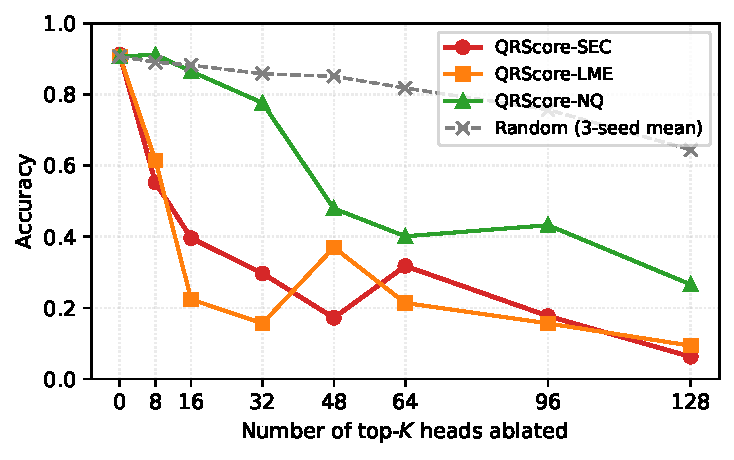
\includegraphics[width=\columnwidth]{figures/fig1_apples_to_apples_llama.pdf}
\caption{Per-method accuracy curves on the Llama-3.1-8B-Instruct $n{=}192$ SEC subset. QRScore-SEC and QRScore-LME ablations cause large drops; QRScore-NQ ablation is statistically indistinguishable from the random baseline at small $K$. The QRScore-LME effect on Llama is much larger than on Qwen or Mistral (\Cref{sec:limitations}). LME and NQ are evaluated on the same $192$ SEC instances to avoid mixing baselines.}
\label{fig:apples}
\end{figure}

QRScore-SEC ablation reduces Llama accuracy from $91.1\%$ to $39.6\%$ at $K{=}16$ on the $192$-instance SEC subset---a $51.6$ percentage point drop. Random ablation at the same $K$ averages a $2.4$pp drop across three seeds (\Cref{fig:apples}). The replication on Qwen-2.5-7B-Instruct ($n{=}241$, $K{=}16$) shows a $55.2$pp drop; Mistral-7B-Instruct-v0.3 ($n{=}192$) a $37.0$pp drop. The pooled SEC ablation effect is therefore robust across the three models.

The cross-task transfer matrix shows that this effect is broadly distributed within each model. On Llama at $K{=}16$, $6$ of $8$ specificity indices are non-positive, and bootstrap $95\%$ CIs exclude zero for $4$ of those $6$ (\Cref{app:specificity}). Knocking out one task's top-$16$ heads damages other tasks as much as or more than the source task itself. Within a model, retrieval heads behave as a shared substrate, not as per-task circuits.

\subsection{Asymmetric cross-model conservation}
\label{sec:asymmetry}

\begin{figure*}[!t]
\centering
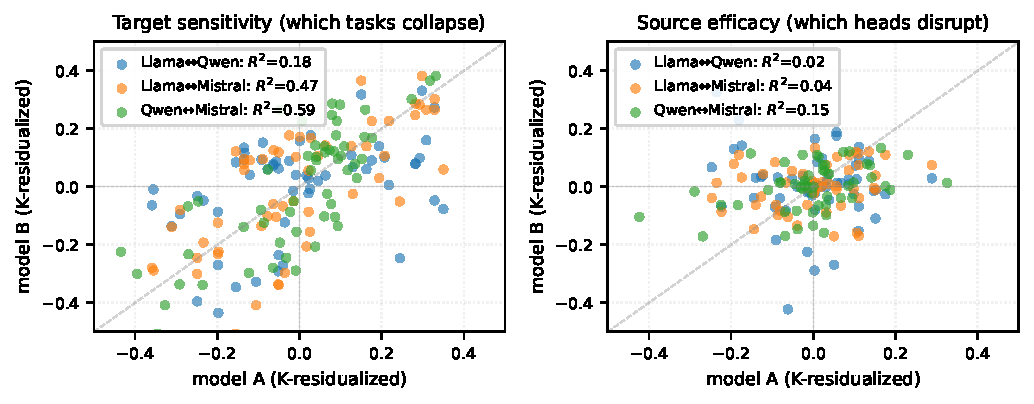
\includegraphics[width=0.92\textwidth]{figures/fig2_kfe_asymmetry.pdf}
\caption{$K$-residualized cross-model correlations of (left) target sensitivity, the per-task column mean of the drop matrix, and (right) source efficacy, the per-task off-target row mean. Each point is one (task, $K$) cell. Target sensitivity correlates substantially across all three model pairs ($R^2 = 0.18$--$0.59$); source efficacy is essentially uncorrelated ($R^2 \leq 0.15$). The asymmetry in $R^2$ is $4$--$12\times$. Full breakdown in \Cref{app:kfe}.}
\label{fig:kfe}
\end{figure*}

The headline result of this paper is the asymmetry visible in \Cref{fig:kfe}. After $K$-residualization, the per-task target sensitivity vectors of two models correlate at $R^2 = 0.18$ (Llama-Qwen), $0.47$ (Llama-Mistral), and $0.59$ (Qwen-Mistral). The matching source efficacy vectors correlate at $R^2 = 0.02$, $0.04$, and $0.15$. The ratio of conserved-target to conserved-source $R^2$ is between $4\times$ and $12\times$ across pairs. \textit{Which target tasks collapse} under any $16$-head ablation is significantly cross-model conserved; \textit{which source-task heads do the disrupting} is not.

This asymmetry is not a numerical artefact of the residualization. Of the four candidate efficacy definitions enumerated in \Cref{app:kfe-defs}, the two pure off-target measures (\texttt{off\_target\_mean} and the full row mean, the latter dominated by off-target cells) both give cross-model $R^2 \leq 0.16$. The two definitions that incorporate the on-target drop $\Delta_{s\to s}$ (\texttt{on\_target\_drop} alone, and the specificity index) give higher cross-model $R^2$ precisely because they partially re-express the conserved target sensitivity. \texttt{off\_target\_mean} is the canonical efficacy used here, with values reproducing the headline asymmetry within $|\Delta| = 0.0035$.

\subsection{Cross-model head pools do not overlap above chance}
\label{sec:not-shared}

\begin{figure}[!htbp]
\centering
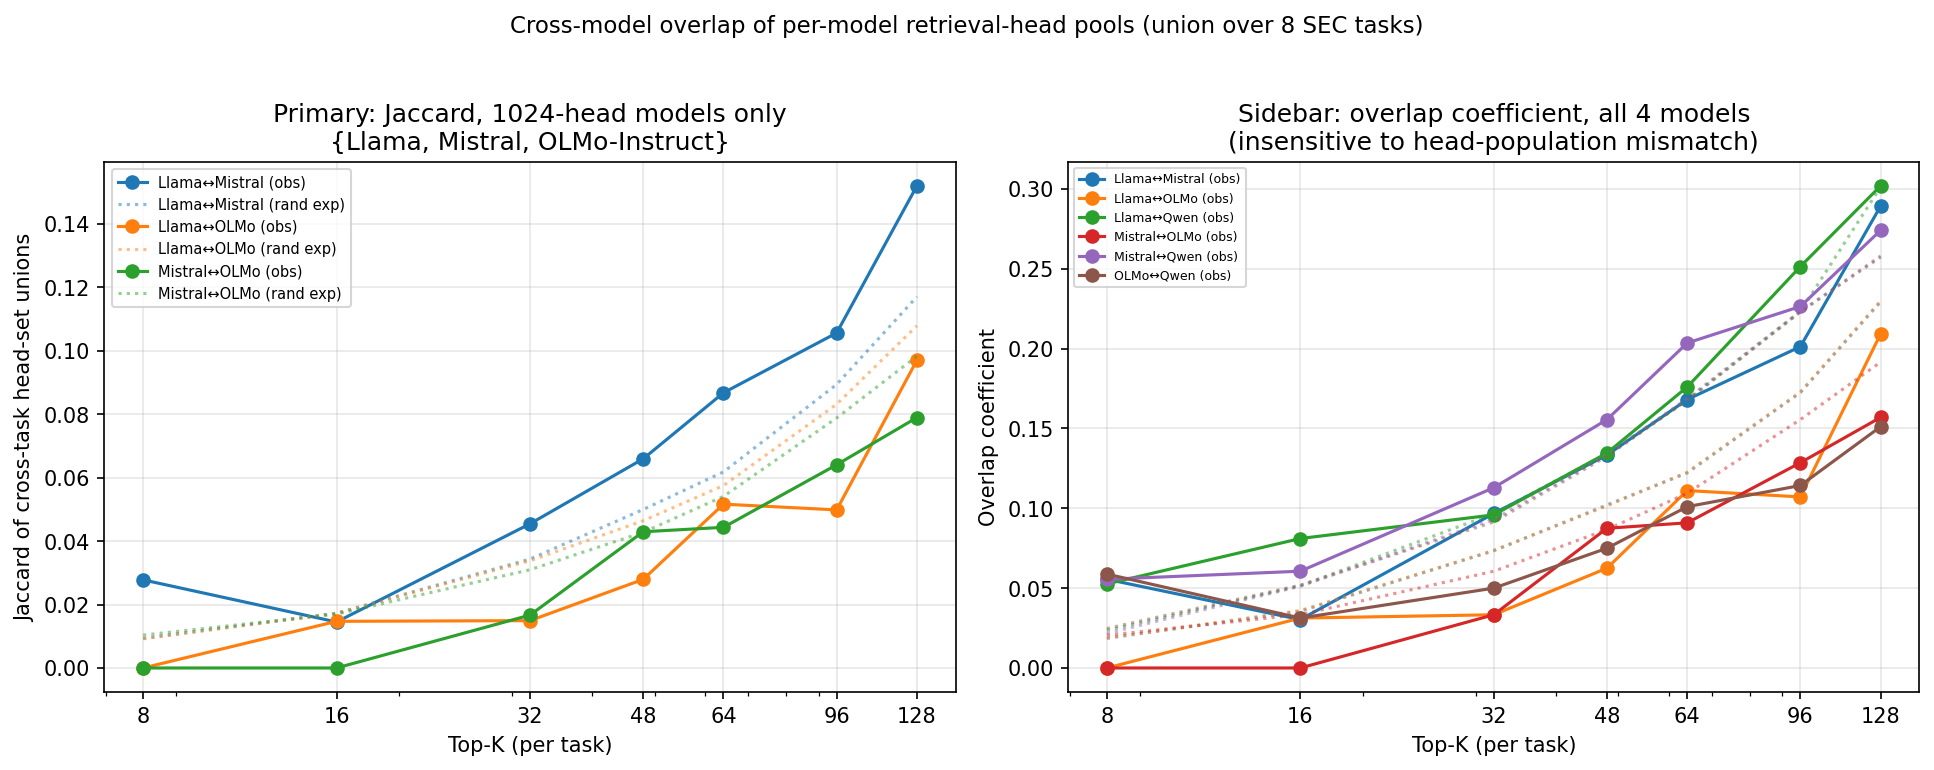
\includegraphics[width=\columnwidth]{figures/cross_model_union_overlap_plot.png}
\caption{Cross-model union-overlap of per-model retrieval-head pools $U_M(K) = \bigcup_t \mathcal{H}^{(t)}_K$. \textbf{Left}: Jaccard for matched-population pairs (Llama / Mistral / OLMo-Instruct, all $1024$ heads). \textbf{Right}: overlap coefficient for all four models including Qwen ($784$ heads). Dotted lines are empirical random expectation from $1000$ random subset pairs. At $K{=}16$, observed lifts above random are $0.0\times$--$1.7\times$ across pairs.}
\label{fig:overlap}
\end{figure}

If the conserved target sensitivity in \Cref{fig:kfe} reflected a shared physical substrate of heads, we would expect cross-model retrieval-head pools to overlap above random expectation. They do not (\Cref{fig:overlap}). At $K{=}16$, the Jaccard of $U_{\text{Llama}} \cap U_{\text{Mistral}}$ is $0.014$ against a random expectation of $0.017$ (lift $0.8\times$, one-sided $p{=}0.69$). Similar values hold for all other pairs. The conservation observed in \Cref{fig:kfe} is therefore not driven by shared head identity. \emph{Models implement retrieval with different heads but agree on which tasks are vulnerable.}

\subsection{Predicting fragility from task structure, not difficulty}
\label{sec:predictors}

If conserved fragility were merely a re-expression of conserved task difficulty, fragility should track baseline accuracy. It does not: the cross-model fragility-vs-baseline-accuracy correlation is $r = -0.09$ ($p = 0.83$, $n=8$). Tasks with high baseline accuracy can be either fragile (\taskpill{employees\_count\_total}, baseline $0.93$, fragility $0.69$) or robust (\taskpill{registrant\_name}, baseline $0.96$, fragility $0.11$); the fragility hierarchy is not a difficulty hierarchy.

A simple structural feature does correlate. The median word-distance from a task-keyword's first occurrence in the haystack to the answer's first occurrence is strongly negatively associated with fragility: $r = -0.72$, $p = 0.04$ Pearson; $\rho = -0.71$, $p = 0.05$ Spearman (scatter plot in \Cref{app:predict-fig}). Tasks where the answer is far from query keywords (e.g., \taskpill{headquarters\_state} at distance $856$, fragility $0.22$; \taskpill{registrant\_name} at $519$, fragility $0.11$) are robust to ablation. Tasks where the answer sits close to the query keyword (e.g., \taskpill{employees\_count\_total} at distance $64$, fragility $0.69$; \taskpill{ceo\_lastname} at $9$, fragility $0.43$) are fragile. We interpret this as evidence that close-attention retrieval relies on a more concentrated head population, while distance-spanning retrieval is more distributed and therefore more redundant. The correlation should be read as suggestive given $n{=}8$ tasks; it is reported here because it survives a Bonferroni-style adjustment for the three tested predictors only on the Pearson side ($p = 0.04 \times 3 = 0.13$, marginal).

\section{Limitations}
\label{sec:limitations}

\paragraph{Ablation only.} We measure the population-level effect of head removal on accuracy. We do not perform causal patching, attention-pattern decomposition, or feature-level analysis, and we therefore do not claim circuit-level understanding. Following \citet{sharkey2025openproblems} we use ``head population'' and ``substrate'' rather than ``circuit.'' All four models are $7$--$8$B parameters\textcolor{red}{ [three end-to-end + OLMo overlap-only --- consider rephrasing to avoid the overclaim]}; whether the asymmetry persists at frontier scale is open.

\paragraph{Statistical power.} Cross-task correlations use $n{=}8$ tasks; the predictive-fragility correlation in \Cref{sec:predictors} (scatter in \Cref{app:predict-fig}) is $p = 0.04$ before multiple-comparison correction. We treat \Cref{sec:predictors} as suggestive rather than confirmatory.

\paragraph{Mixed and negative results.} \Cref{fig:apples} shows a $68$pp effect from LME-detected heads on Llama; the same heads cause a $\sim 3$pp drop on Qwen and a $\sim 15$pp drop on Mistral. Cross-paradigm transfer is therefore model-dependent, and we do not claim the LME-vs-NQ ``two-paradigm'' story as a finding (per-model numbers in \Cref{app:lme-nq}). We also tested whether fragile-task heads concentrate in different layers than robust-task heads (per-task layer entropy, permutation test on fragile-vs-robust difference); permutation $p \geq 0.107$ across all five models analysed (\Cref{app:layer}). A direct random-source-head null distribution would strengthen \Cref{fig:kfe} but requires GPU runs that were not completed for this submission. The existing $3$-seed random ablation in \Cref{fig:apples} provides a partial substitute.

\section{Conclusion}

In four open-weights $7$--$8$B language models\textcolor{red}{ [three with full ablation pipeline; OLMo overlap-only --- same overclaim as in abstract/intro/limitations]}, retrieval-head ablation evidence is consistent with the following picture: each model has a within-domain shared retrieval substrate, the substrates differ in their physical head identities across models, but the resulting task-vulnerability hierarchy is preserved. The hierarchy is not a difficulty hierarchy and is partially predicted by within-document query-to-answer distance. We take this as a small piece of evidence that long-context fact extraction is \textcolor{red}{implementation-variant [defend ``implementation'' or soften? reviewer flag]} but task-structurally constrained. The open mechanistic question is what, beyond retrieval distance, makes specific tasks structurally fragile under any retrieval-head intervention.

\clearpage

\bibliography{refs}
\bibliographystyle{icml2026}

\newpage
\appendix
\onecolumn

\section{Models and benchmark details}
\label{app:models}

\begin{table}[h]
\centering
\small
\begin{tabular}{lrrrr}
\toprule
\textbf{Model} & \textbf{Layers} & \textbf{Q heads/layer} & \textbf{KV heads/layer} & \textbf{Total Q heads} \\
\midrule
Llama-3.1-8B-Instruct      & 32 & 32 & 8  & 1024 \\
Mistral-7B-Instruct-v0.3   & 32 & 32 & 8  & 1024 \\
OLMo-7B-Instruct           & 32 & 32 & 32 & 1024 \\
Qwen2.5-7B-Instruct        & 28 & 28 & 4  & 784 \\
\bottomrule
\end{tabular}
\caption{Model architectural statistics. Query heads are the units of ablation.}
\end{table}

\paragraph{Per-model evaluation set sizes.} Llama: $n{=}192$ ($24/\text{task}$). Qwen: $n{=}241$ (per-task counts $24$--$41$). Mistral: $n{=}192$. OLMo: head-identity analysis only, no ablation pipeline. The per-method comparison in \Cref{fig:apples} restricts LME and NQ accuracy to the $192$ Llama SEC instances to avoid mixing baselines.

\paragraph{Reproducibility.} All ablation results were generated by an end-to-end head-knockout pipeline that registers forward pre-hooks on each layer's $o_{\text{proj}}$, zeroing out the slices corresponding to ablated heads. Per-model detection JSONs (top-$K$ heads per task) drive the ablation. The $K$-fixed-effects analysis flattens each model's drop matrix to a $56$-element vector after subtracting within-$K$ task means, and reports Pearson $R^2$ across model pairs.

\section{$K$-fixed-effects table and definition shootout}
\label{app:kfe}
\label{app:kfe-defs}

\Cref{tab:kfe-full} reports cross-model Pearson $R^2$ after $K$-residualization for one sensitivity definition and four candidate efficacy definitions. The residualization formula is unambiguous (subtract within-$K$ task means; flatten; Pearson $R^2$). Only \texttt{off\_target\_mean} reproduces values reported in a prior version of the paper to within $|\Delta| \leq 0.05$.

\begin{table}[h]
\centering
\small
\begin{tabular}{llccc}
\toprule
\textbf{Measure} & \textbf{Definition} & \textbf{Llama-Qwen} & \textbf{Llama-Mistral} & \textbf{Qwen-Mistral} \\
\midrule
Sensitivity & column mean of drop matrix     & 0.184 & 0.472 & 0.593 \\
Efficacy    & off-target row mean              & 0.018 & 0.039 & 0.153 \\
Efficacy    & full row mean (incl.\ on-target) & 0.054 & 0.002 & 0.096 \\
Efficacy    & on-target drop only              & 0.031 & 0.332 & 0.302 \\
Efficacy    & specificity index ($-$off-target) & 0.133 & 0.466 & 0.434 \\
\bottomrule
\end{tabular}
\caption{$K$-residualized cross-model $R^2$. Sensitivity values and the \texttt{off\_target\_mean} efficacy values reproduce the headline numbers reported in \Cref{sec:asymmetry} within $|\Delta| \leq 0.0035$. The other three efficacy definitions diverge from \texttt{off\_target\_mean} by total $|\Delta|=0.13$--$0.82$ on the published reference table; the best-matching definition (\texttt{off\_target\_mean}) is identified by minimum total absolute deviation.}
\label{tab:kfe-full}
\end{table}

A verification harness asserts that all six rows reproduce within $\text{EPS}=0.05$ of the published reference values (set at $\sim 2\times$ the published two-significant-figure quantization to be tolerant of minor numpy/scipy version drift).

\section{Per-task specificity with bootstrap CIs (Llama)}
\label{app:specificity}

\begin{table}[h]
\centering
\small
\begin{tabular}{lrrrr}
\toprule
\textbf{Source task} & \textbf{On-target drop} & \textbf{Off-target mean} & \textbf{Specificity} & \textbf{$95\%$ CI} \\
\midrule
\taskpill{headquarters\_city}      & 0.50  & 0.52  & $-0.02$ & $[-0.23, +0.21]$ \\
\taskpill{headquarters\_state}     & 0.21  & 0.63  & $\mathbf{-0.42}$ & $[-0.57, -0.27]$ \\
\taskpill{registrant\_name}        & 0.17  & 0.33  & $\mathbf{-0.17}$ & $[-0.34, -0.02]$ \\
\taskpill{employees\_count\_total} & 0.08  & 0.02  & $\mathbf{+0.06}$ & $[+0.03, +0.09]$ \\
\taskpill{holder\_record\_amount}  & 0.04  & $-0.01$ & $\mathbf{+0.05}$ & $[+0.03, +0.07]$ \\
\taskpill{ceo\_lastname}           & $-0.04$ & 0.04 & $\mathbf{-0.08}$ & $[-0.10, -0.06]$ \\
\taskpill{incorporation\_state}    & 0.00  & 0.03  & $-0.03$ & $[-0.06, 0.00]$  \\
\taskpill{incorporation\_year}     & 0.00  & 0.01  & $-0.01$ & $[-0.04, +0.02]$ \\
\bottomrule
\end{tabular}
\caption{Specificity index = on-target drop $-$ off-target mean drop, at $K{=}16$ on Llama-3.1-8B-Instruct. Negative entries indicate broad collateral damage; bold entries have $95\%$ bootstrap CIs that exclude zero.}
\label{tab:specificity}
\end{table}

\section{Predictive-fragility scatter plots}
\label{app:predict-fig}

\begin{figure}[h]
\centering
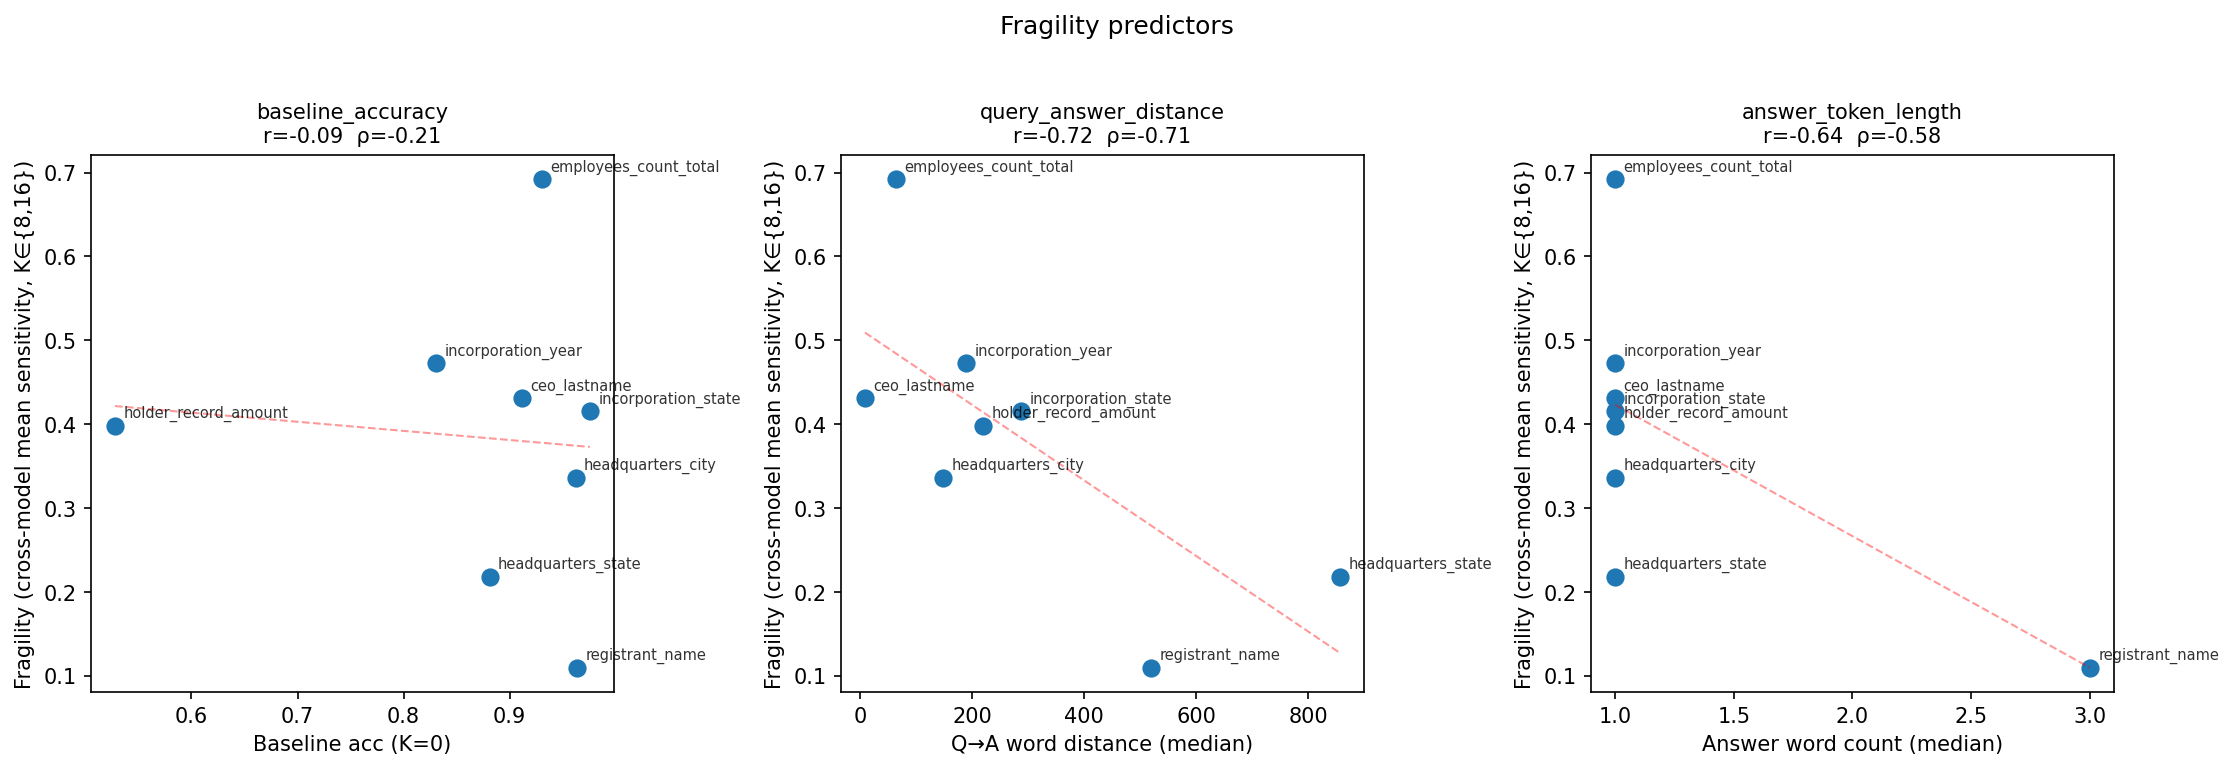
\includegraphics[width=\textwidth]{figures/scatter_plots.png}
\caption{Cross-model fragility (mean target sensitivity across the three models, $K \in \{8, 16\}$) plotted against three candidate predictors. Fragility does not correlate with baseline task accuracy ($r{=}{-}0.09$, $p{=}0.83$) but correlates negatively with within-document query-to-answer word distance ($r{=}{-}0.72$, $p{=}0.04$) and answer token length ($r{=}{-}0.64$, $p{=}0.09$). The eight task labels are visible on each panel.}
\label{fig:predict-app}
\end{figure}

\section{Cross-task transfer heatmap and per-task curves}
\label{app:transfer}

\Cref{fig:transfer-heatmap} shows the source $\times$ target drop matrix on Llama at $K{=}16$, the data underlying the within-model substrate claim in \Cref{sec:within-model}. \Cref{fig:per-task-curves} resolves the same data per target task across the full $K$ sweep.

\begin{figure}[h]
\centering
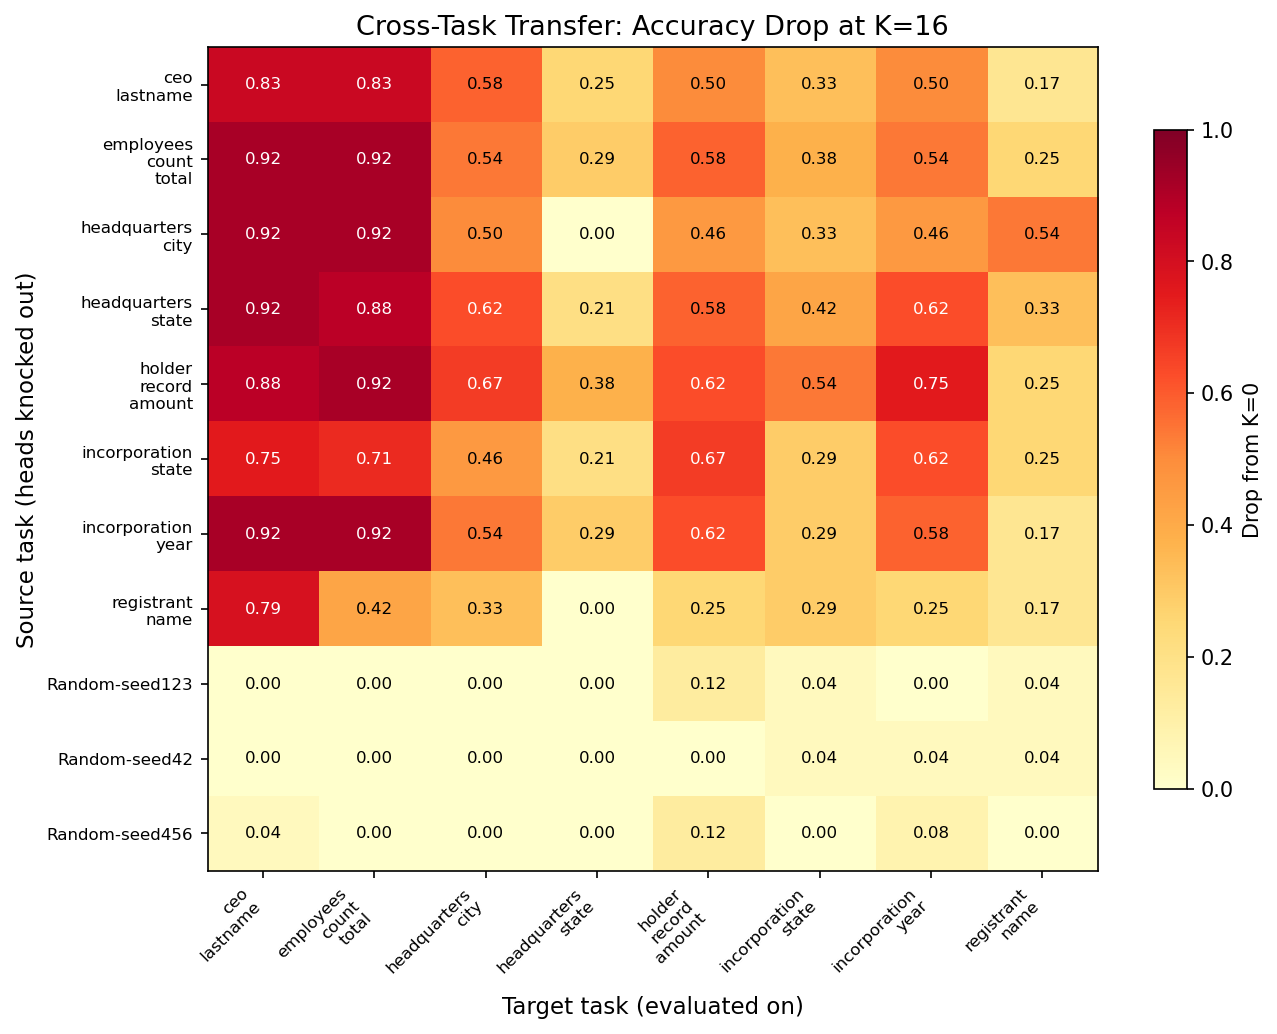
\includegraphics[width=0.62\textwidth]{figures/fig3_llama_transfer_K16.png}
\caption{Cross-task transfer drop matrix at $K{=}16$ on Llama. Rows are source tasks (heads ablated); columns are target tasks (evaluation). Random-seed rows at the bottom serve as the random-ablation control. Off-diagonal cells are typically as red as on-diagonal cells---the substrate effect.}
\label{fig:transfer-heatmap}
\end{figure}

\begin{figure}[h]
\centering
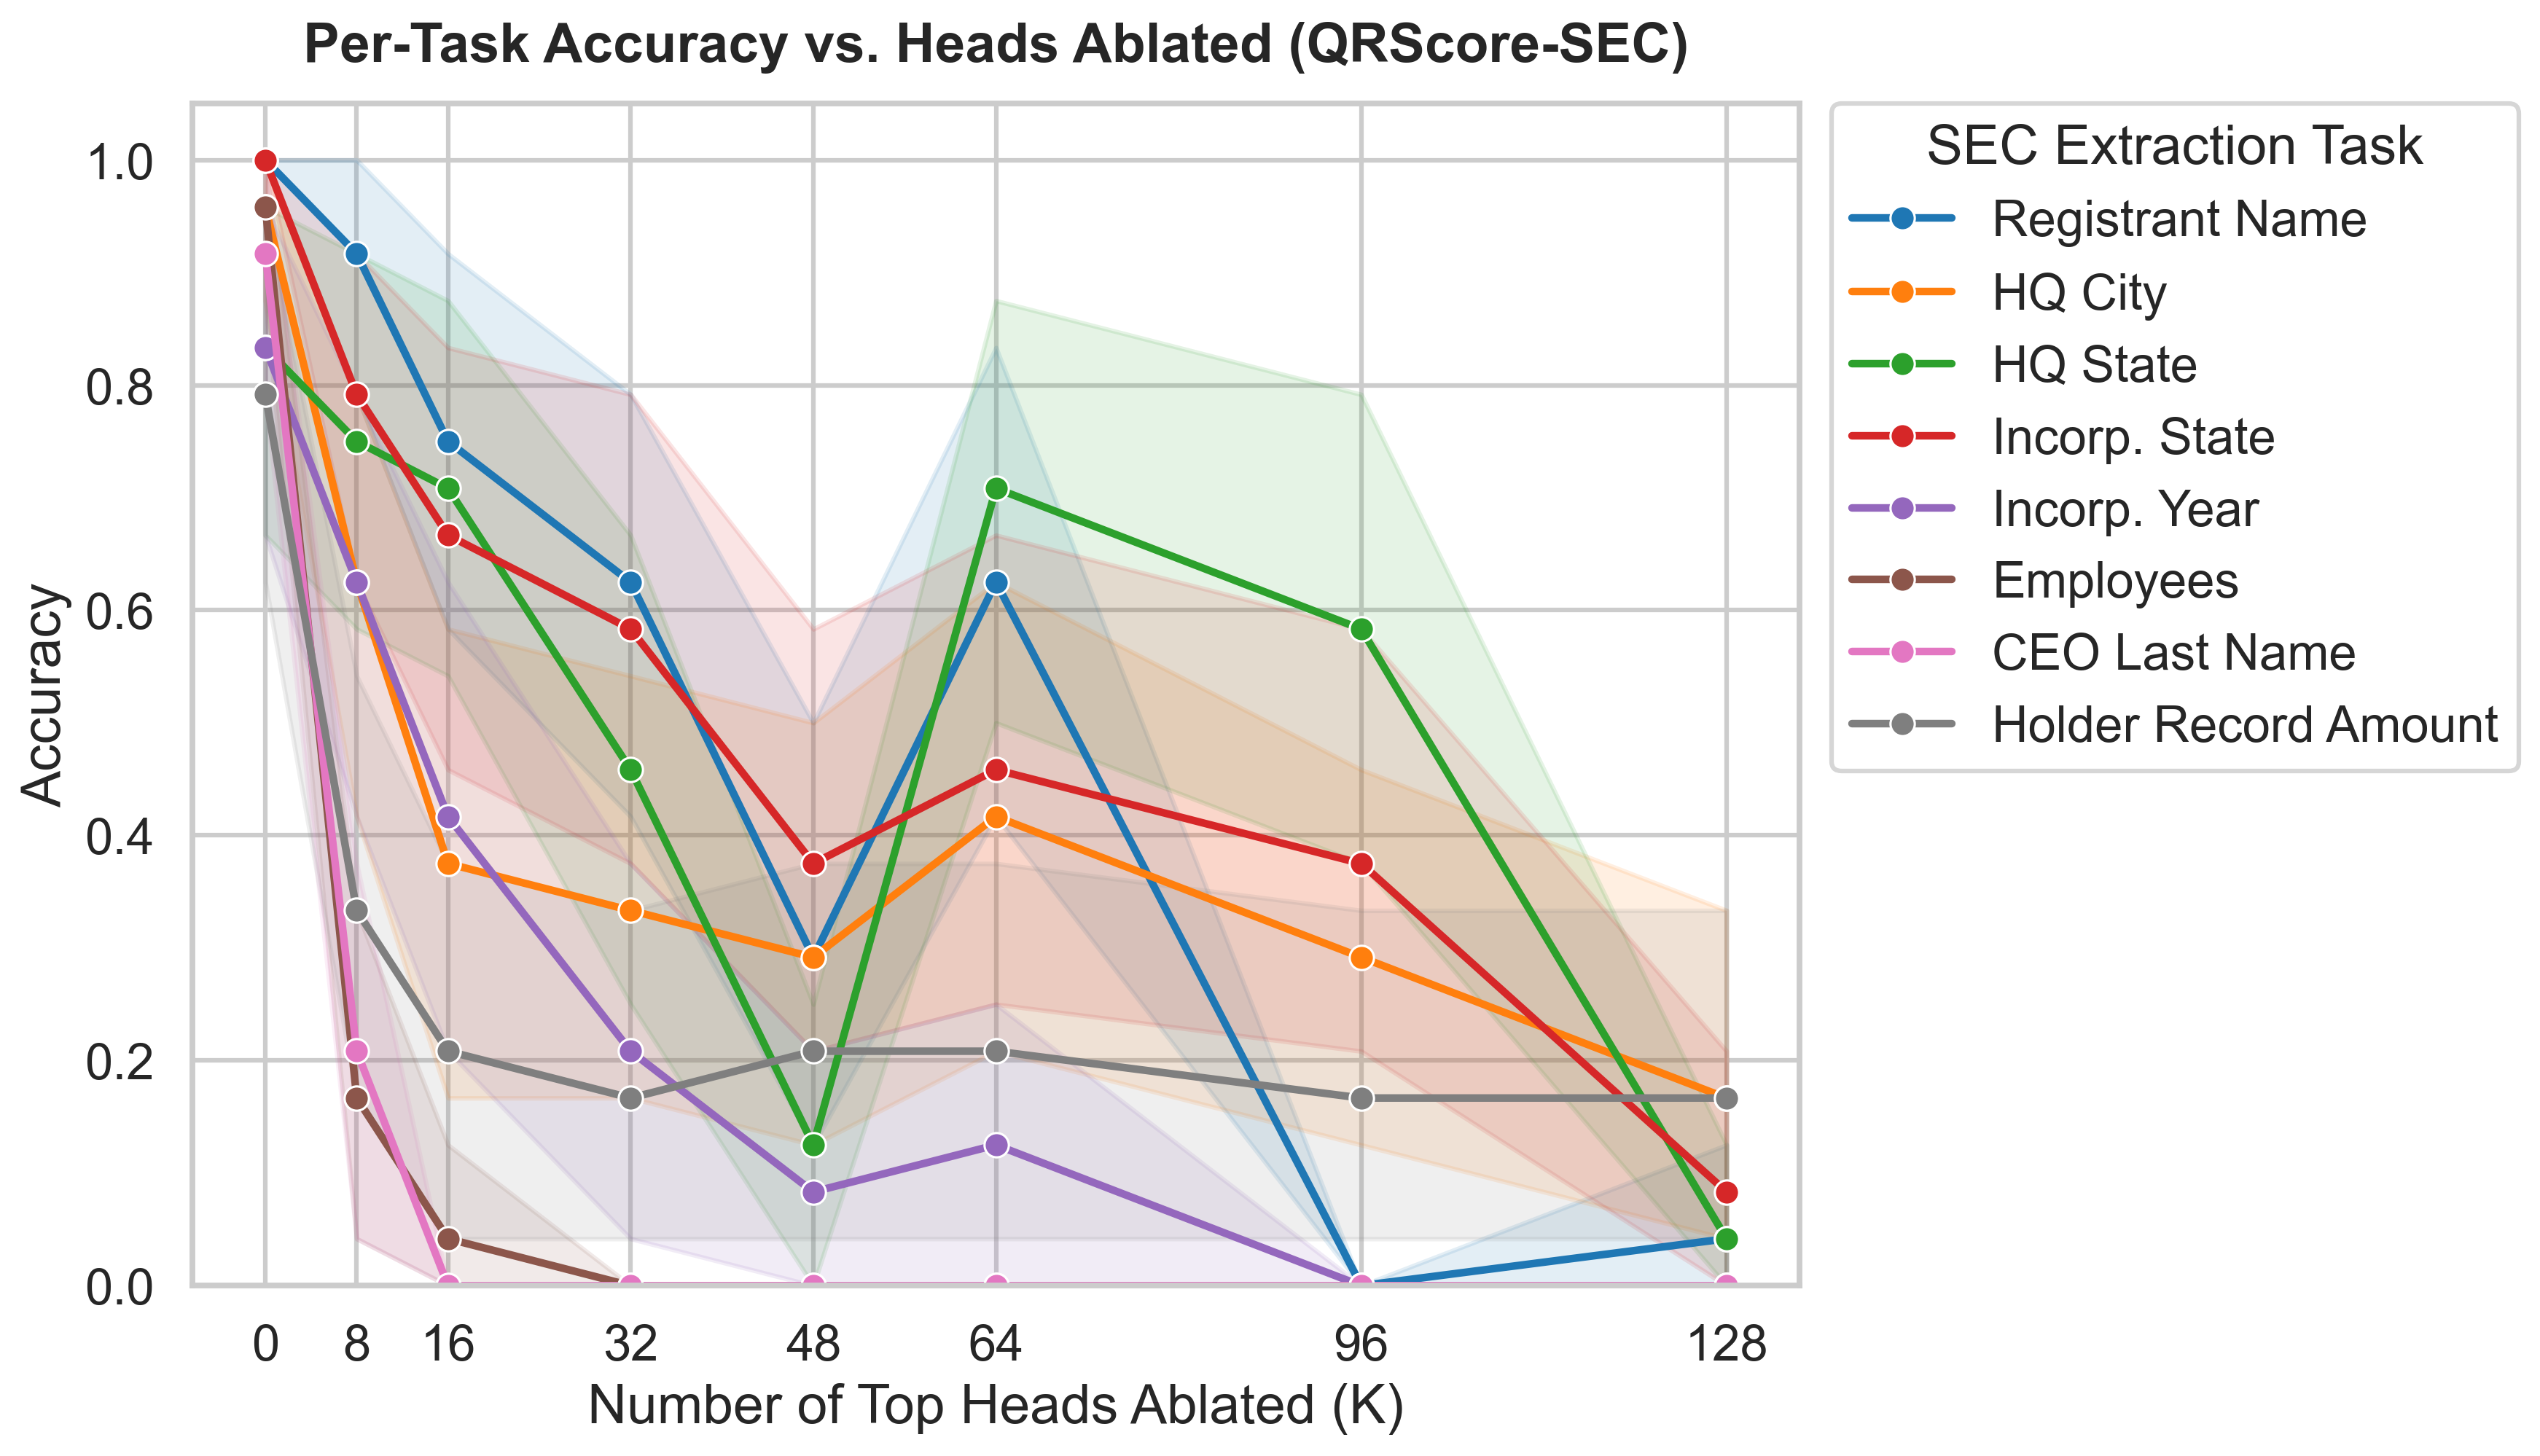
\includegraphics[width=0.85\textwidth]{figures/fig2_llama_per_task_curves.png}
\caption{Per-task accuracy curves for QRScore-SEC ablation on Llama. Shaded bands are bootstrap $95\%$ CIs. Numeric/name tasks (\taskpill{employees\_count\_total}, \taskpill{ceo\_lastname}) collapse rapidly; entity tasks (\taskpill{headquarters\_state}, \taskpill{registrant\_name}) degrade gradually. The $K{=}64$ bump on the pooled curve is sampling noise (Findings note).}
\label{fig:per-task-curves}
\end{figure}

\section{Negative result: layer position does not separate fragile from robust tasks}
\label{app:layer}

\begin{table}[h]
\centering
\small
\begin{tabular}{lrrrr}
\toprule
\textbf{Model} & \textbf{Mean fragile entropy} & \textbf{Mean robust entropy} & \textbf{Permutation $p$} & \textbf{Mann-Whitney $U$ $p$} \\
\midrule
Llama-3.1-8B-Instruct & 1.561 & 1.842 & 0.293 & 0.343 \\
Mistral-7B-Instruct   & 1.900 & 1.882 & 0.840 & 0.885 \\
OLMo-7B-Instruct      & 1.798 & 1.859 & 0.480 & 0.663 \\
OLMo-7B (base)        & 1.526 & 1.399 & 0.107 & 0.108 \\
Qwen2.5-7B-Instruct   & 1.738 & 1.718 & 0.942 & 0.686 \\
\bottomrule
\end{tabular}
\caption{Layer-entropy difference between fragile (top-$4$ by cross-model fragility) and robust (bottom-$4$) tasks. Permutation test ($1000$ random fragile/robust assignments) and Mann-Whitney $U$ on the four-vs-four per-task entropies are both non-significant in all five models. Pooled-KS testing is intentionally avoided (tasks share heads---see \Cref{sec:within-model}---so pooled samples are not independent).}
\label{tab:layer}
\end{table}

\begin{figure}[h]
\centering
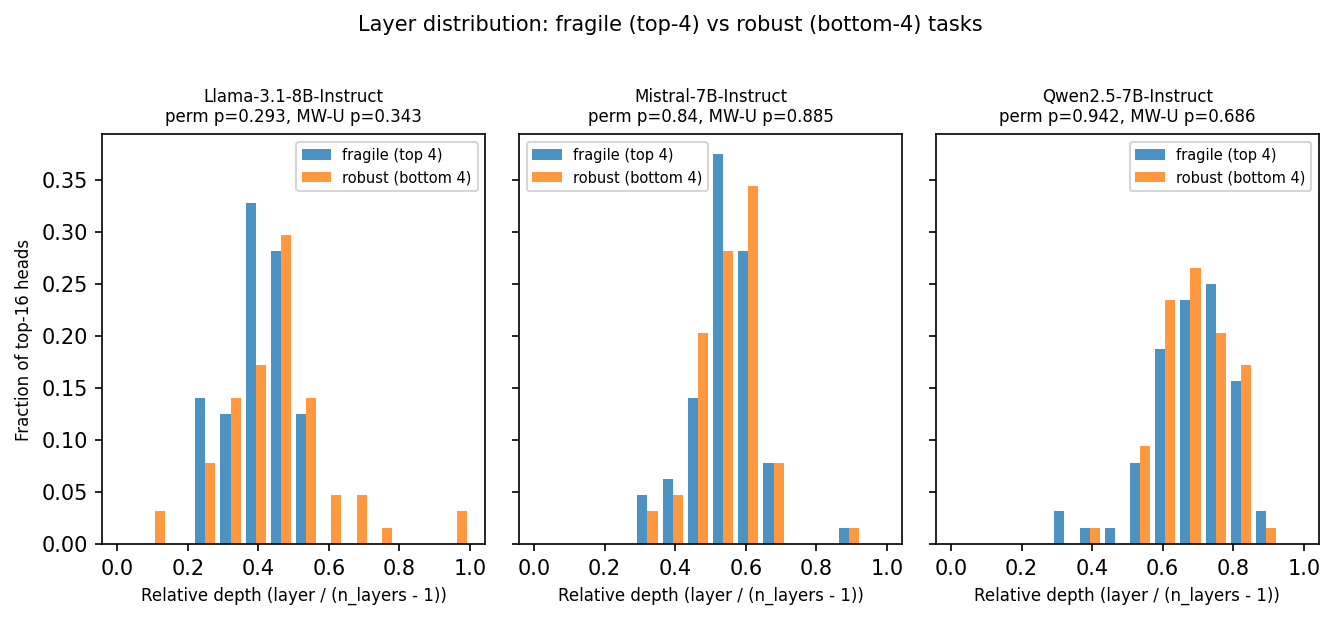
\includegraphics[width=\textwidth]{figures/fragile_vs_robust_overlay.png}
\caption{Fragile (blue) and robust (orange) per-task layer distributions on a relative-depth axis. The two distributions are visually similar within each model. We do not detect a fragility signature in layer position.}
\end{figure}

\section{LME and NQ paradigm transfer is model-dependent}
\label{app:lme-nq}

\Cref{tab:lme-nq} contrasts the per-method drop at $K{=}16$ on the $n{=}192$ SEC subset for QRScore-LME, QRScore-NQ, and the three-seed random baseline across the three models with full pipelines.

\begin{table}[h]
\centering
\small
\begin{tabular}{lrrrr}
\toprule
\textbf{Model} & \textbf{QRScore-SEC} & \textbf{QRScore-LME} & \textbf{QRScore-NQ} & \textbf{Random (3-seed)} \\
\midrule
Llama-3.1-8B-Instruct       & $-51.6$ & $-68.2$ & $-4.2$ & $-2.4$ \\
Qwen2.5-7B-Instruct         & $-55.2$ & $-2.5$  & $-0.8$ & $-0.4$ \\
Mistral-7B-Instruct-v0.3    & $-37.0$ & $-14.6$ & $+1.6$ & $-0.4$ \\
\bottomrule
\end{tabular}
\caption{Drop in accuracy (percentage points) at $K{=}16$, all on the $n{=}192$ SEC subset. The QRScore-NQ effect (passage-sorting paradigm) is at-or-near random across all three models; the QRScore-LME effect varies dramatically by model family. We therefore do not promote the LME-vs-NQ ``two-paradigm'' story to a finding.}
\label{tab:lme-nq}
\end{table}

\section{Cross-model union overlap, all $K$}
\label{app:overlap-all}

\Cref{fig:overlap-all} extends \Cref{fig:overlap} from the body to the full $K$ sweep. Lifts above random rise modestly with $K$ (mechanically, as the per-model unions cover a larger fraction of the head population) but stay $\leq 2\times$ across all $K \in \{8, 16, 32, 48, 64, 96, 128\}$ for every model pair.

\begin{figure}[h]
\centering
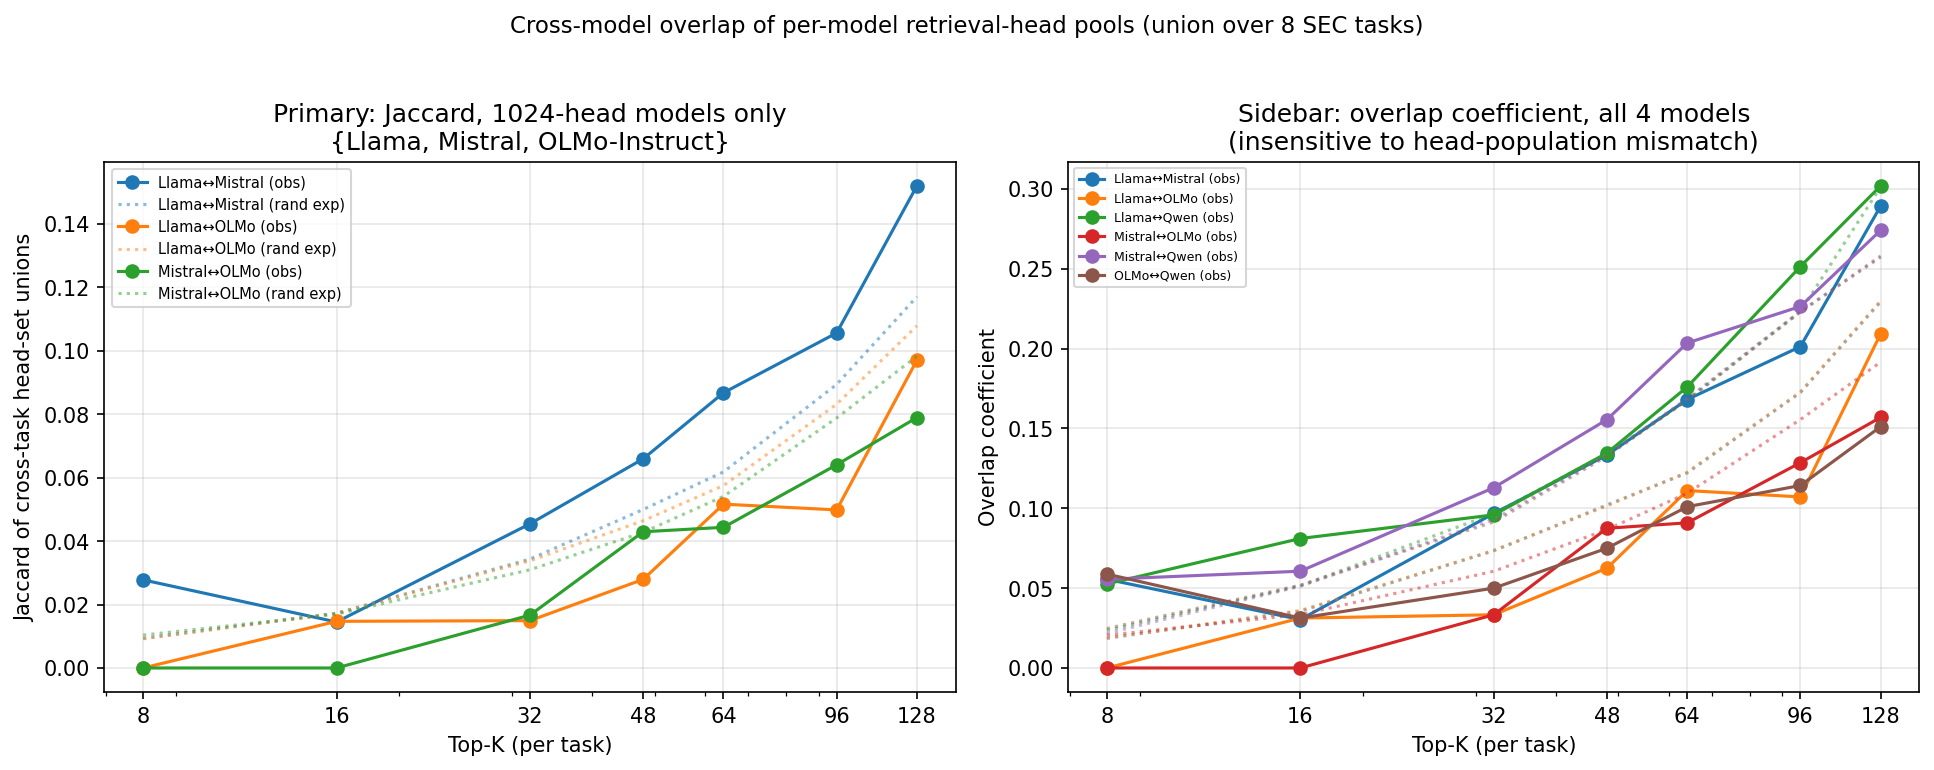
\includegraphics[width=\textwidth]{figures/cross_model_union_overlap_plot.png}
\caption{Full $K$-sweep version of \Cref{fig:overlap}.}
\label{fig:overlap-all}
\end{figure}

\section{Geographic head sub-cluster}
\label{app:cluster}

\Cref{fig:cluster} shows per-task head-set Jaccard at top-$K$ on Qwen-2.5-7B-Instruct. The \taskpill{headquarters\_city} / \taskpill{headquarters\_state} / \taskpill{registrant\_name} sub-cluster is visible at small $K$ (top-$16$ Jaccard $\geq 0.45$ among that triple) and recurs in Llama (top-$16$ \taskpill{HQ-city} $\leftrightarrow$ \taskpill{HQ-state} $J{=}0.78$) and Mistral. We treat this as a small mechanistic supporting result for the within-model shared pool in \Cref{sec:within-model}, not a headline.

\begin{figure}[h]
\centering
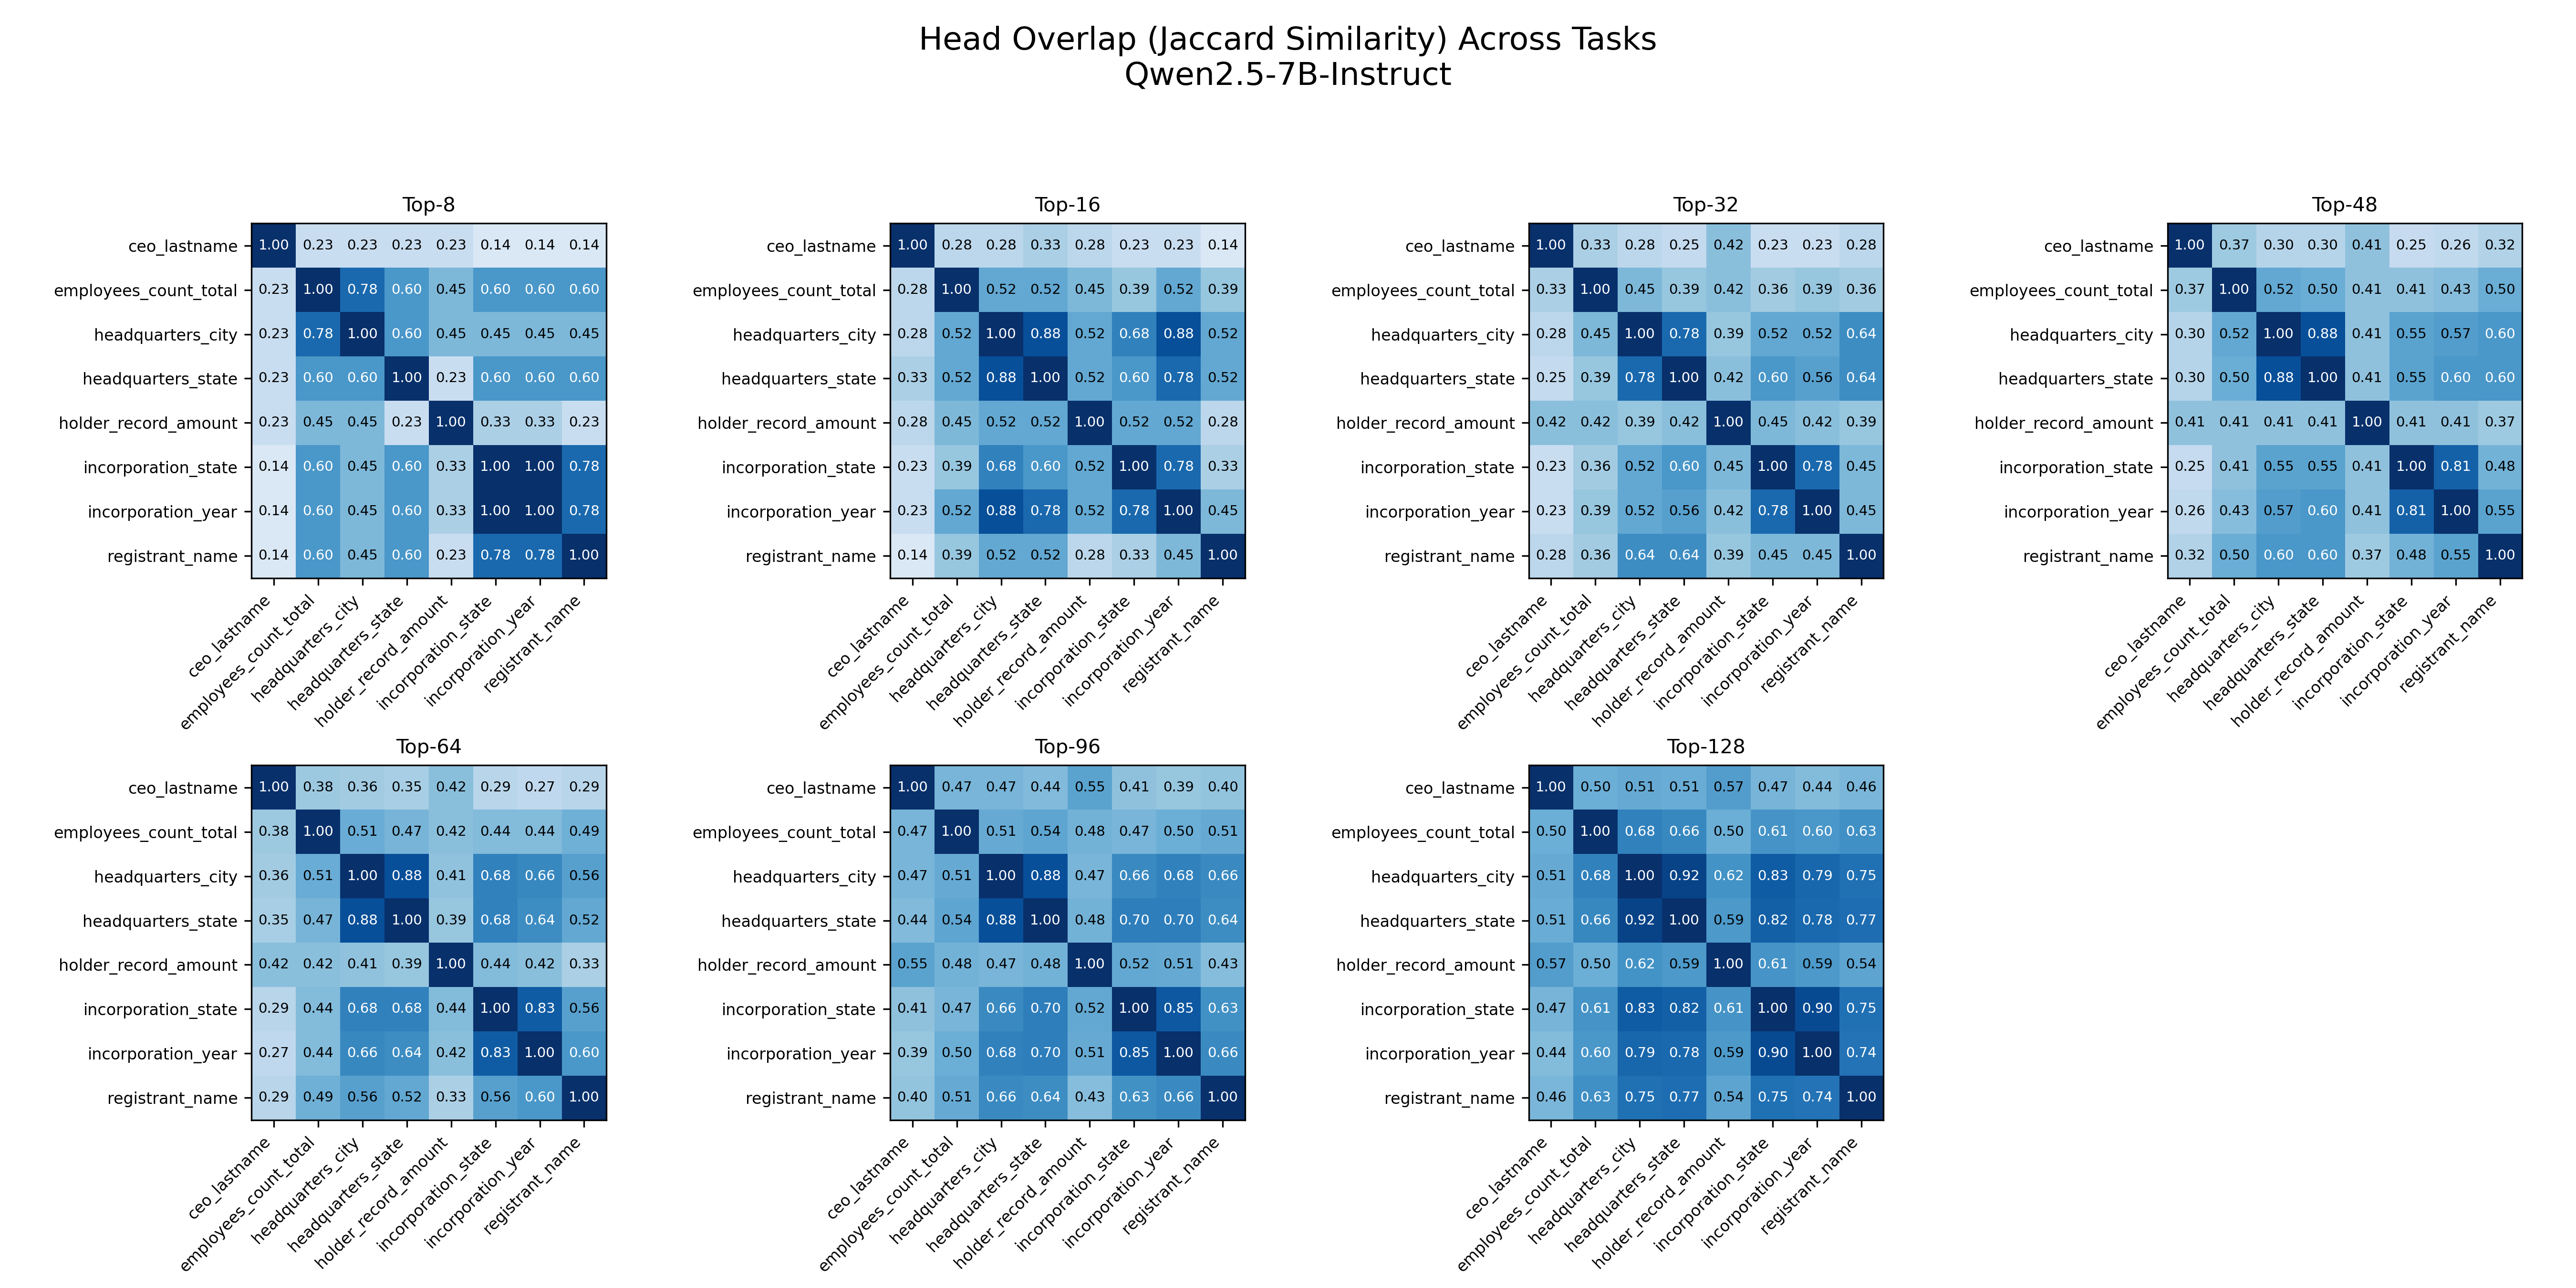
\includegraphics[width=0.85\textwidth]{figures/fig6_qwen_head_similarity.png}
\caption{Per-task Jaccard at top-$K$ on Qwen-2.5-7B-Instruct. The \taskpill{headquarters\_city} / \taskpill{headquarters\_state} / \taskpill{registrant\_name} sub-cluster (top-$16$ Jaccard $\geq 0.45$) is visible at small $K$. The same sub-cluster appears on Llama (top-$16$ \taskpill{HQ-city} $\leftrightarrow$ \taskpill{HQ-state} $J{=}0.78$) and Mistral. We treat this as a small mechanistic supporting result for the within-model substrate, not a headline.}
\label{fig:cluster}
\end{figure}

\section{Reproducibility}

The full pipeline is straightforward to reproduce given the four open-weights models and the EDGAR-CORPUS source filings. Steps:

\begin{enumerate}
\itemsep0pt
\item \textbf{Build the benchmark.} Sample $\geq 24$ filings per task from EDGAR-CORPUS, hold out a leakage-controlled split, and construct each evaluation instance by inserting the gold section at the haystack midpoint with distractor sections drawn from the same filing.
\item \textbf{Detect retrieval heads.} For each (task, model) pair, run QRScore: aggregate post-softmax attention from query tokens to gold-evidence chunks, rank all heads by total mass, take the top-$K$ slice for $K \in \{8, 16, 32, 48, 64, 96, 128\}$.
\item \textbf{Ablate.} Register forward pre-hooks on each layer's $o_{\text{proj}}$ that zero out the slices corresponding to ablated heads. Evaluate on every (source-task heads, target-task instances) pair to populate the $8 \times 8 \times |K|$ drop tensor.
\item \textbf{$K$-residualize and correlate.} For each per-task summary (target sensitivity = column mean, source efficacy = off-target row mean), subtract within-$K$ task means, flatten to a $56$-element vector, and report Pearson $R^2$ across model pairs.
\item \textbf{Cross-model overlap.} For each model $M$ form $U_M(K) = \bigcup_t \mathcal{H}^{(t)}_K$; report Jaccard for matched-population pairs and the overlap coefficient for mixed-population pairs; compare to the empirical random expectation from $1000$ random subset pairs.
\end{enumerate}

Random-baseline ablations use seeds $\{42, 123, 456\}$. All bootstrap CIs use $10{,}000$ task-resamples.

\section*{Impact statement}
This paper presents work whose goal is to advance the field of mechanistic interpretability. There are many potential societal consequences of advances in interpretability for deployed language models, none of which we feel must be specifically highlighted here.

\end{document}